\chapter{Experiment setup}
\lhead{Experiment setup}
\rhead{Radu-George Rusu}
\label{ExperimentSetup}

This chapter will present the thought process and the setup that was used to run the experiments on the dataset presented in Chapter \ref{DatasetChapter}.

\section{Initial idea}

Taking a high level look through the training data set, a general case can be seen: pictures are taking at sea (no port in site) and as such, they are also conceived from water and ships (which can divide pixels in two group as shown in image \ref{ShipExampleAtSea}). If the images are moved into grayscale, and its histogram is computed (\ref{ImageHistogram}), then the pixels of the image can be split into two groups, which will also give the ship/no-ship classification. This problem is classical problem that can be solved using EM algorithm.

\begin{figure}[h]
	\centering
	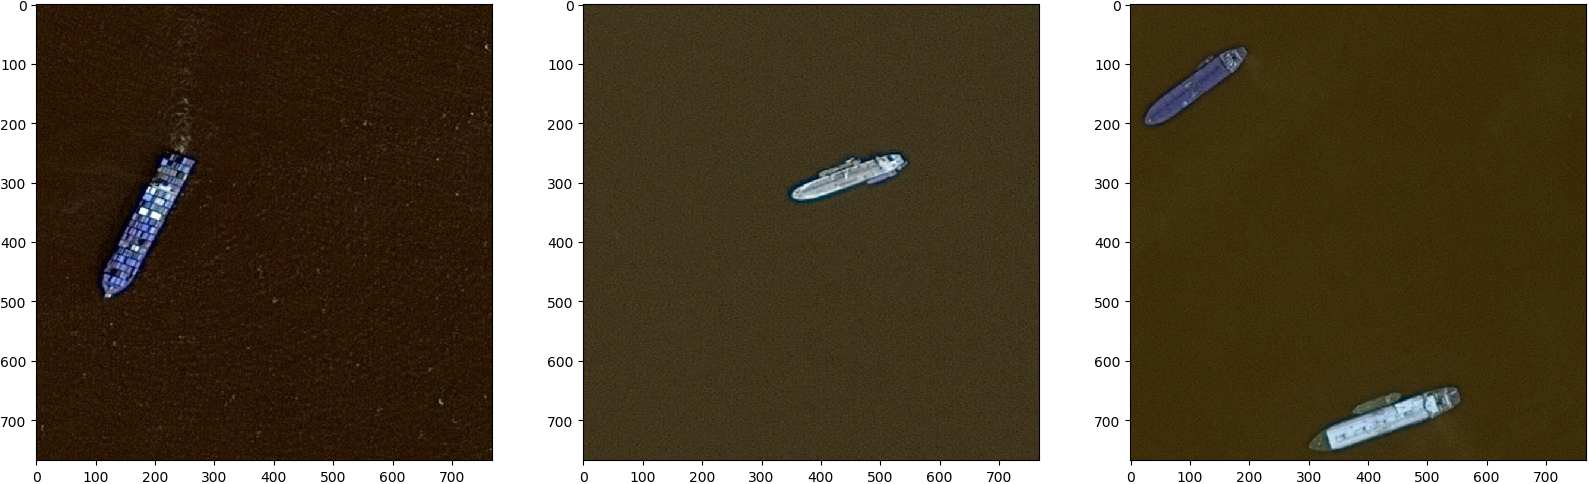
\includegraphics[height=0.2\textheight]{Pictures/002ShipExampleatSea.png}
	\caption{Ships at sea}
	\label{ShipExampleAtSea}
\end{figure}

\begin{figure}[h]
	\centering
	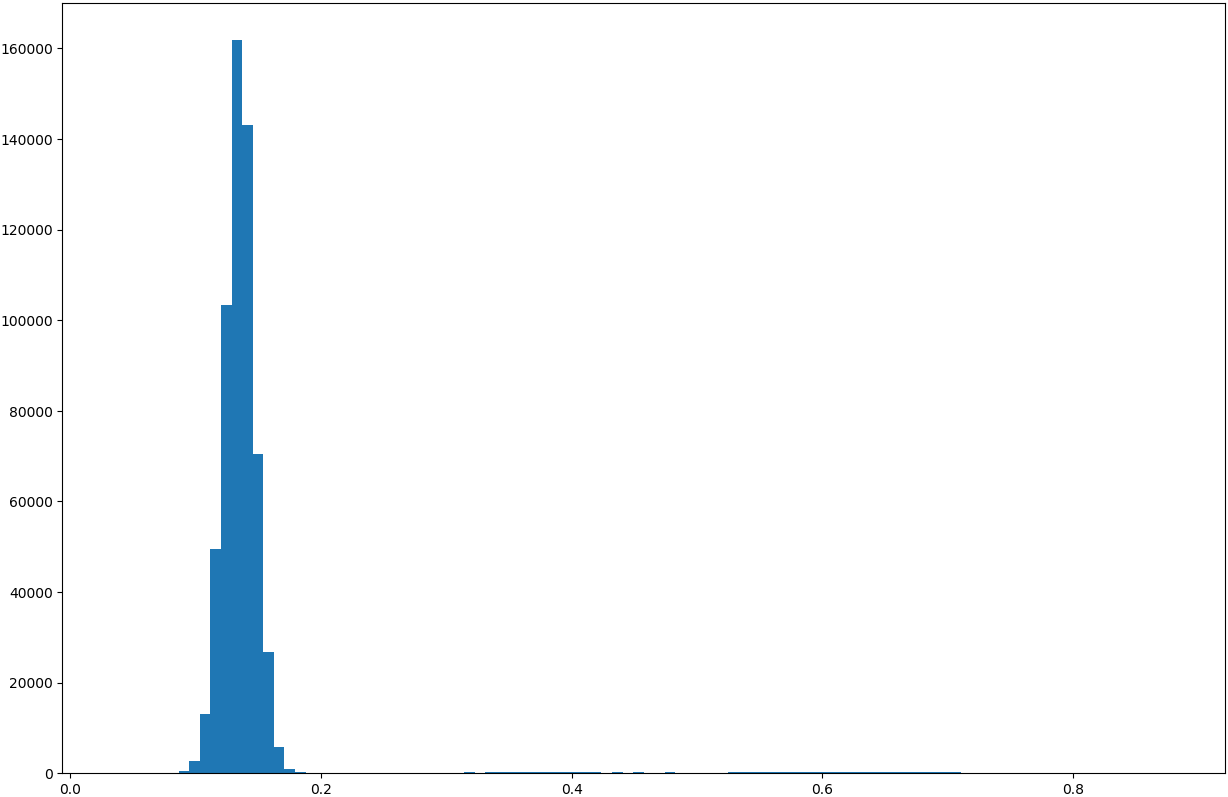
\includegraphics[width=\textwidth]{Pictures/005ImageHistogram.png}
	\caption{Histogram of grayscale at sea image}
	\label{ImageHistogram}
\end{figure}

\subsection{Expectation-Maximization}

\subsubsection{Intuition}


\subsection{Limitations}